\section{Level description}

The city is loosely based on Venice.

\begin{center}
  \begin{figure}[H]
    \centering
    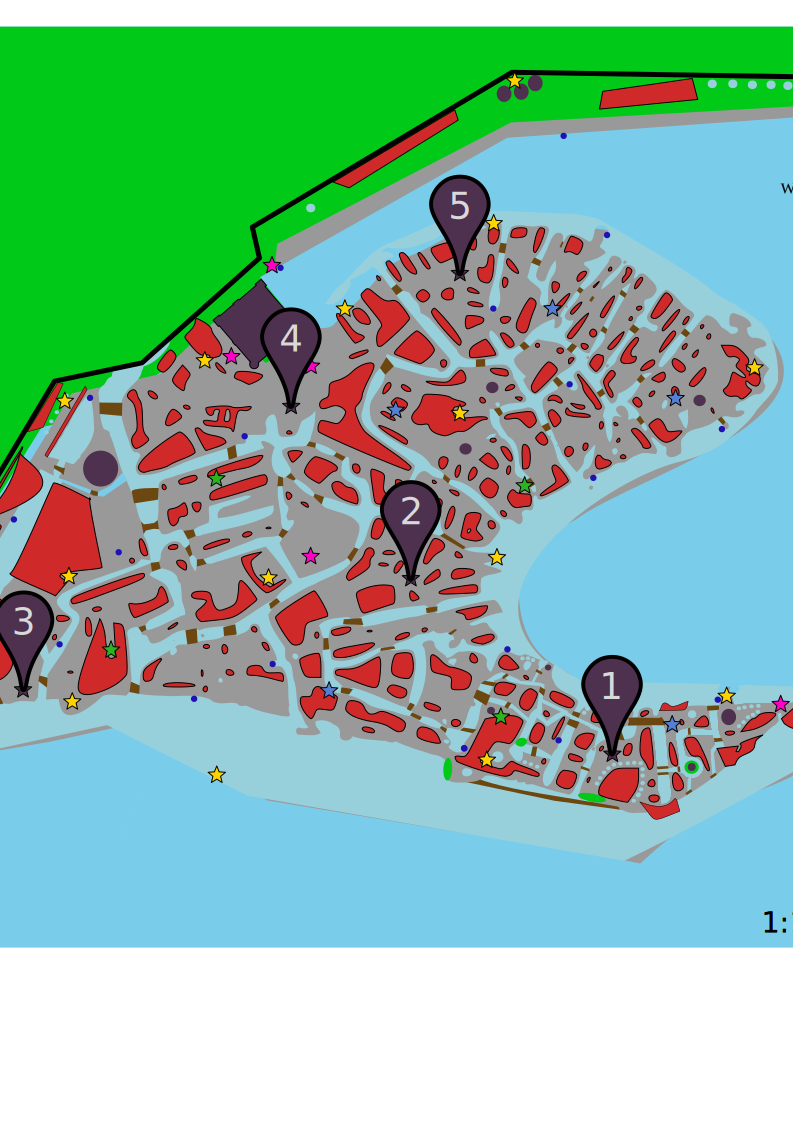
\includegraphics[width=\textwidth]{Images/Maps/dynamia}
    \caption{Map of Dynamia}
  \end{figure}
\end{center}

aaa

\pagebreak

\subsection{Castle of Dynamia}
The castle of Dynamia is loosely based on the Sforza Castle of Milan.

\begin{center}
  \begin{figure}[H]
    \centering
    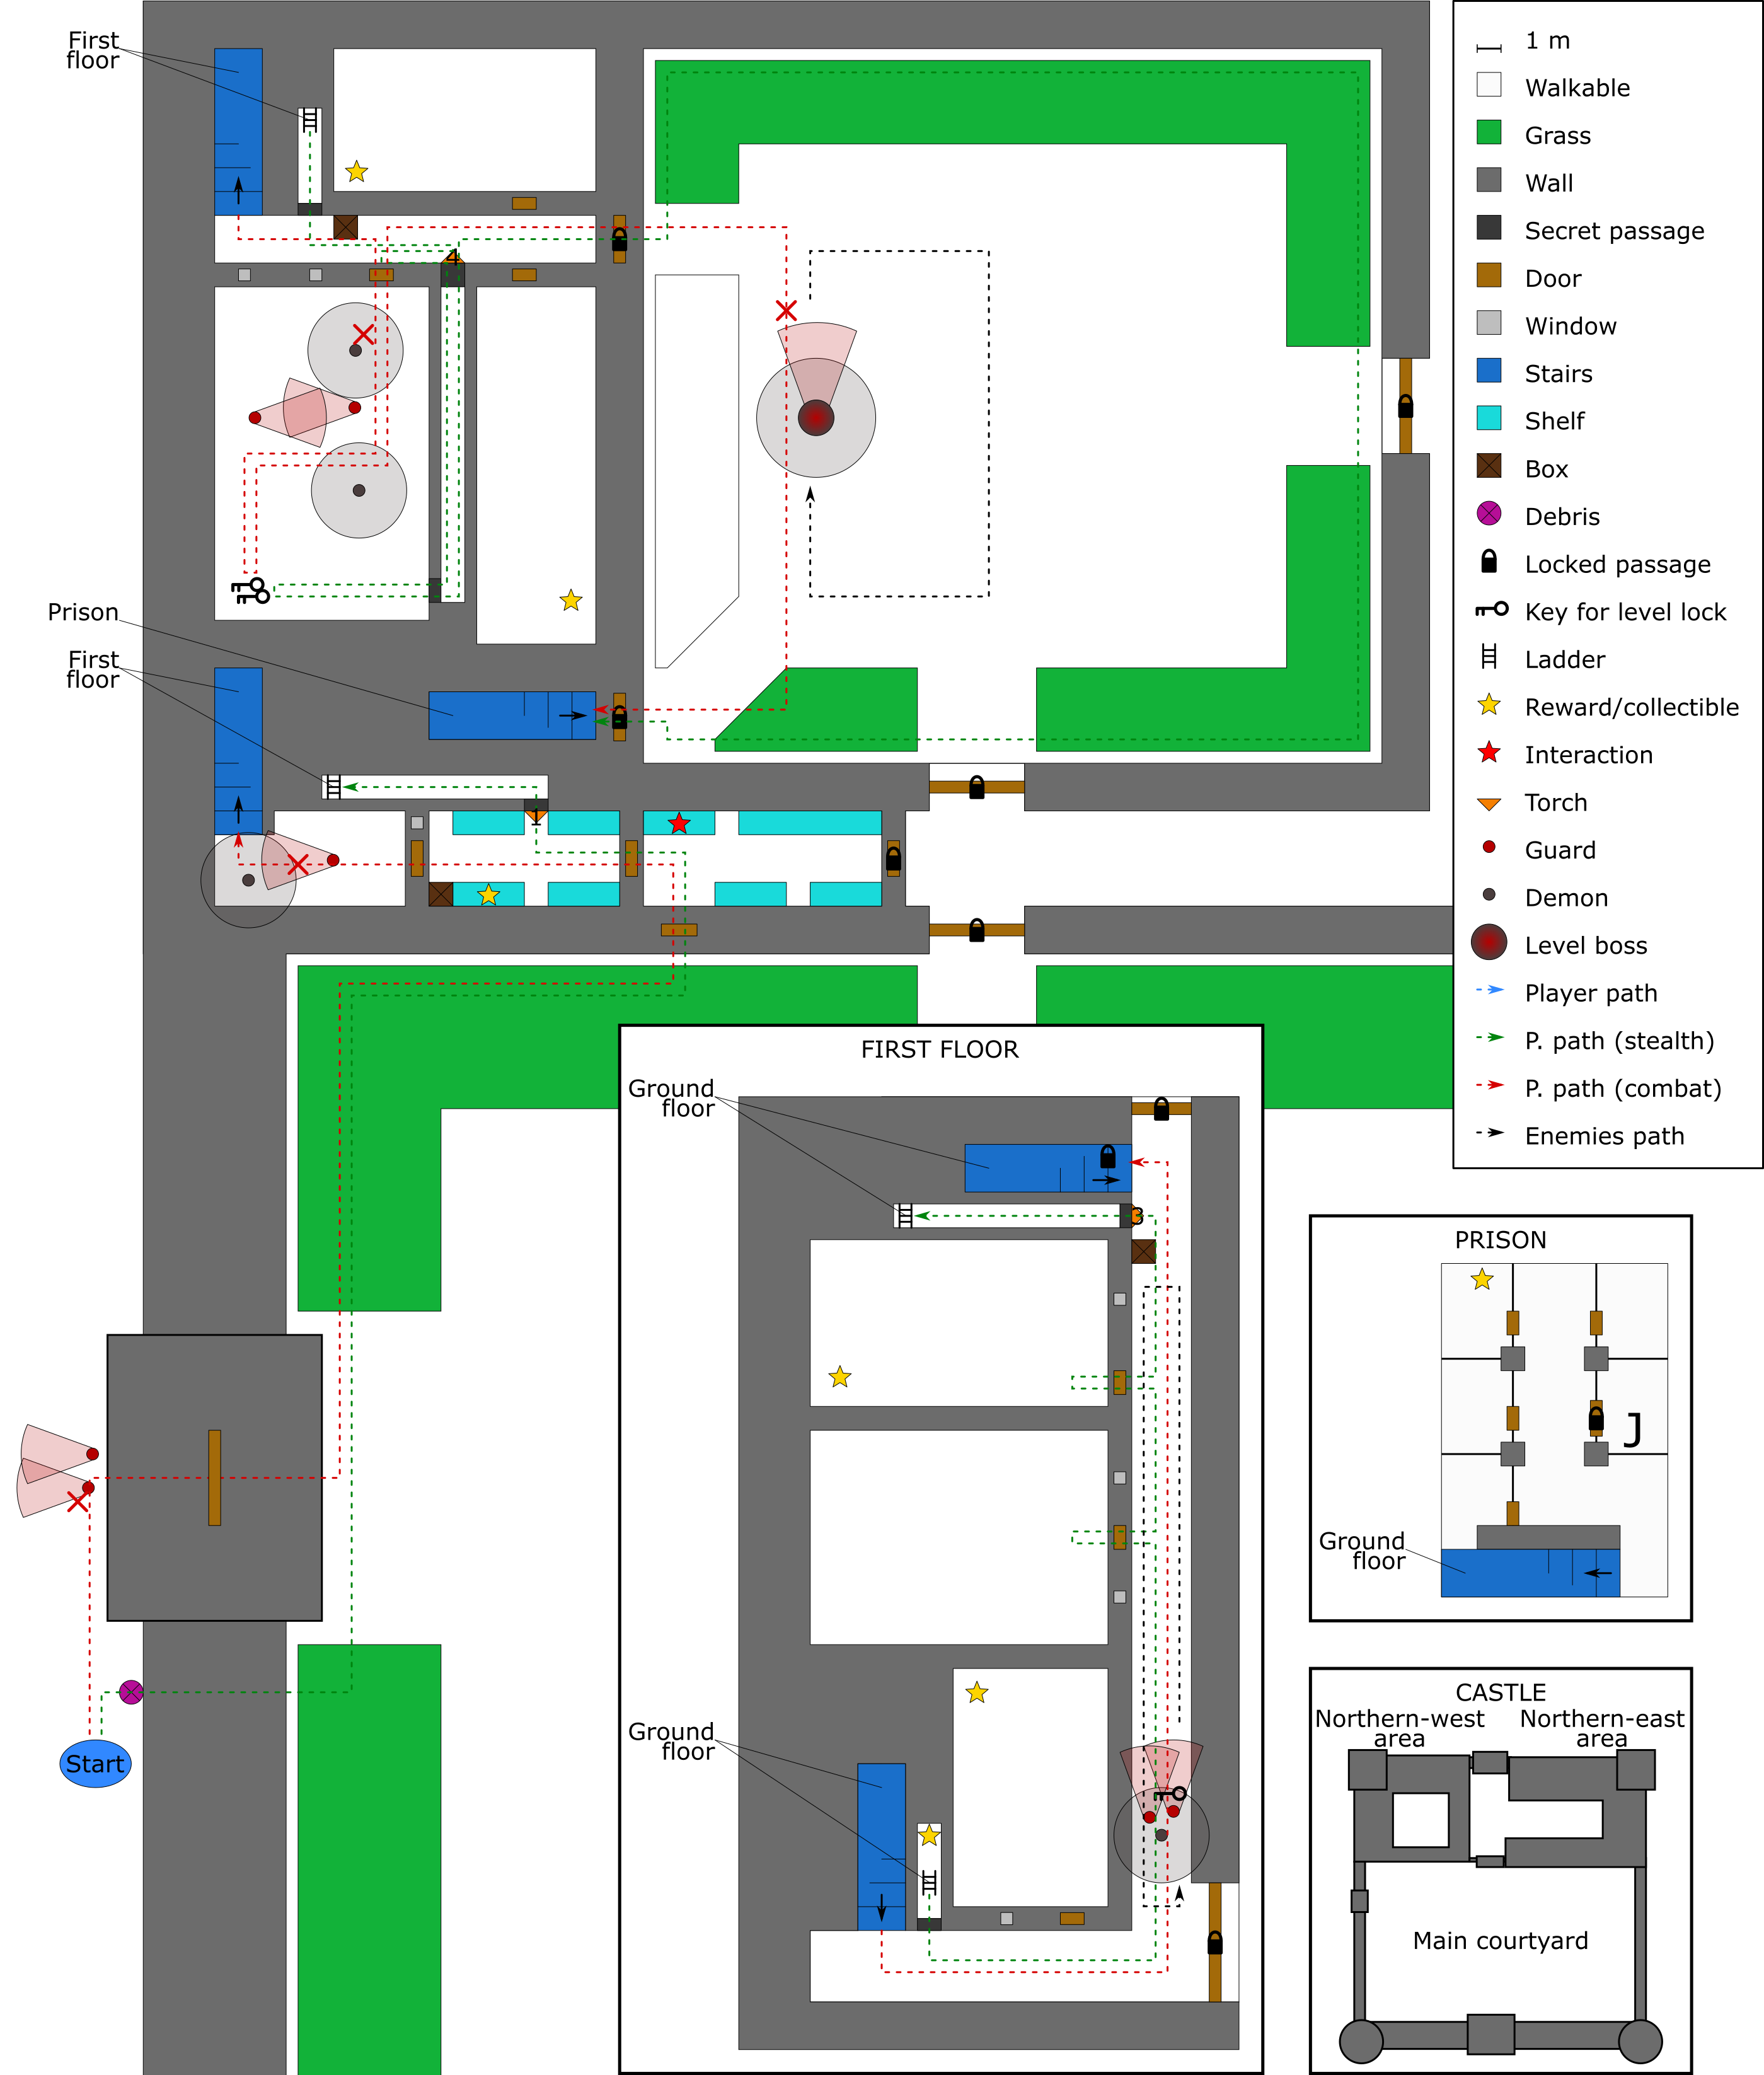
\includegraphics[width=\textwidth]{Images/Maps/castleOfDynamia}
    \caption{Map of the Castle of Dynamia}
  \end{figure}
\end{center}

It is placed upon a rocky promontory and it is the main entrance to Dynamia from the continent. It has been designed by the court magician of Dynamia centuries ago, and it has many secret passages. The player can access some of this secret passages by solving puzzles.

It is made of stones, it has a big courtyard and two buildings: one on the west, heavily fortified, and one, more refined, on the north for the royal family. Mizar lives in the northern building, but the player can visit only the courtyard and the western area.

There are human guards and demons that patrol the castle. They are ordered to arrest any intruder. The most powerful enemy is the captain of the guards.

\subsubsection{Puzzles}
While exploring the castle, the player can choose to solve some puzzles and, by so, avoid fighting some enemies. \\

\textbf{1. Build a construct}

In order to enter in the courtyard the player can use some debris to build a construct for Calcifer that allows him to climb the wall without being detected.

The player has different parts and he/she has to understand how to combine them.\\

\textbf{2. Rotate the torch}

The torch is a puzzle itself. The player has to rotate the torch and its parts according to the given scheme. When the player rotate a block, the upper blocks rotate too according to the scheme in figure X.Y.\\

\textbf{3. Press the bricks}

Near the torch there is a small plate with some horizontal lines. The player has to press the bricks in the corresponding position under the torch.\\

\textbf{4. Connect the cables}

There are some cables that hang under the torch. The player has to connect them in the correct pairs, according to the pattern on the plugs.
